
\section{Prefix Sum Solution (optimized brute force)}
A dynamic programming-styled approach can help us optimize our naive solution using the prefix sum technique. In the previous solution, note that once the two endpoints of the array have been determined, we loop over each of the elements inside the given range and add up their values. This innermost for loop is why our naive solution has complexity $O(n^3)$ and if we are able to access the sum of a given range of elements in constant time, then we can create an $O(n^2)$ solution\footnote{The innermost part of the two nested for loops will run in $O(1)$ time as the only two operations being performed are accessing the sum (which will be in $O(1)$ using the prefix sum technique) and taking the maximum of the global and local answer - both $O(1)$ operations. Hence, the overall complexity for the algorithm will be $O(n \times n) = O(n^2)$, accounting for the two nested for loops.}. This is exactly what the prefix sum technique will allow us to do. \\

\noindent The prefix sum technique involved preprocessing an array and saving cumulative sums to a new array which can be accessed later. We begin by rigorously defining a prefix array that will be used in further computation.  

\noindent \newline \fbox{%
    \parbox{\textwidth}{%
        \textbf{Definition 2} 
        $$\texttt{prefix[k]} = \sum_{i=1}^k \texttt{arr[i]}$$
    }%
}

\noindent \newline A simpler way of stating this mathematical equation is saying that the $\texttt{k}$th number in the \texttt{prefix} array will be the sum of the first $\texttt{k}$ elements from the given array. Now that we know this, we may wonder, how does this help with anything? How is summing the first $\texttt{k}$ elements for each particular index going to allow me to access the sum of a range of particular elements? Indeed. Let's take an example and look at how and why this works. \newline

\noindent Consider the following situation - we have an array of a certain size $\texttt{n}$ and we wish to calculate the sum of the elements between elements $\texttt{i}$ and $\texttt{j}$. Basically, we wish to calculate  $\sum_{k=i}^j \texttt{arr[k]}$ \noindent and our given a \texttt{prefix} array s.t. Definition 2 is satisfied. The question remains - how do we go about doing this with our \texttt{prefix} array?

% insert diagram showing i and j and how we can compute it 
% draw the original array with values arr_i and arr_j at two ends (highlighted)
\begin{center}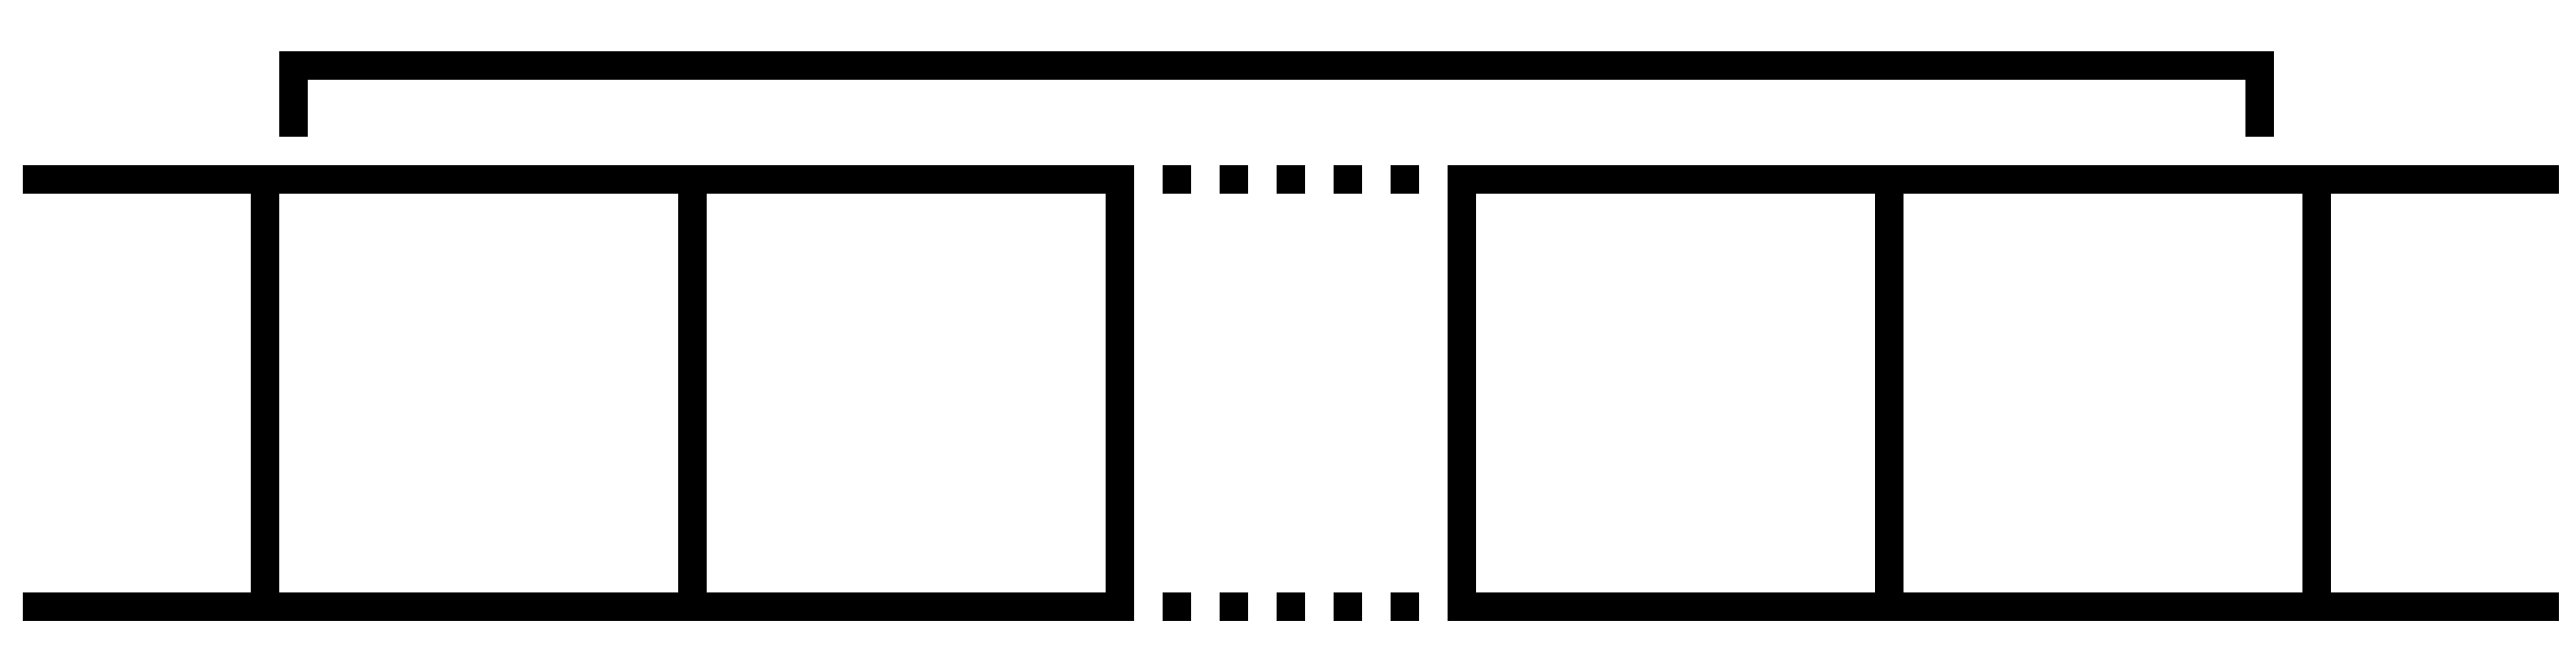
\includegraphics[scale=0.1]{diagram1.png}\end{center}
% have the image working but was unable to put the text in it 

\noindent A useful observation will help us see how we can compute this. Our desired sum is 
$$\sum_{k=i}^j \texttt{arr[k]} = \texttt{arr[i] + arr[i+1] + \dots + arr[j-1] + arr[j]}$$

\noindent Manipulating this equation, we get 

$$\sum_{k=i}^j \texttt{arr[k]} = 
\sum_{k=1}^j \texttt{arr[k]} - \sum_{k=1}^{i-1} \texttt{arr[k]}$$

\noindent Basically, what we're doing is summing all of the values s.t. $\texttt{k} \in [1, \texttt{j}]$ and then subtracting those off s.t. $\texttt{k} \in [1, \texttt{i})$ - effectively meaning that the sum only accounts for those elements that are in the desired range of $[\texttt{i}, \texttt{j}].$ \newline 

\noindent Now, we can use Definition 2 to connect our summations back to the idea of the \texttt{prefix} array:

$$\Rightarrow \texttt{prefix[m]} = \sum_{n=1}^m \texttt{arr[n]}\footnote{We've changed the looping variables from the original definition to prevent any confusion in naming because of contextual differences between the definition's use of looping variables and the current proof.}$$
$$\therefore \sum_{k=1}^j \texttt{arr[k]} = \texttt{prefix[j]} \texttt{ and } \sum_{k=1}^{i-1} = \texttt{prefix[i-1]}$$

\noindent Thus, rewriting our original expression, we have 

$$\sum_{k=i}^j \texttt{arr[k]} = \texttt{prefix[j]} - \texttt{prefix[i-1]}$$

\noindent Thus, after preprocessing a \texttt{prefix} array, we can access the sum of any range of elements in the array in $O(1)$ time directly through subtraction. Now that we've determined how to use our \texttt{prefix} array, let's take a look at how we should approach implementing it. There are two ways we can do this - one direct and one a bit more subtle. Let's take a look at the direct way of computing the sum first. \\

\noindent \textbf{Method 1:} nested for loops \\ 

\noindent We know that for the $\texttt{i}^\text{th}$ element of the \texttt{prefix} array, we need to sum the first $\texttt{i}$ elements. Let's go ahead and do this.

\begin{algorithm}
\caption{}\label{prefix}
\begin{algorithmic}[1]
\Procedure{PSA1}{arr[n+1]}\Comment{one-based indexing; actual elements of the array begin at index 1}
\State $\vars{maxi} \gets -\infty$ 
\State Declare an array $\vars{prefix}$ of size $n+1$.
\State $\vars{prefix[0]} \gets \vars{0}$ 
\For{$\vars{i} \gets 1, n$} 
    \State $\vars{sum} \gets 0$
    \For{$\vars{j} \gets 1, i$} 
        \State $\vars{sum := sum + arr[j]}$
    \EndFor
    \State $\vars{prefix[i] = sum}$
\EndFor
\For{$\vars{i}\gets 1, n$}
    \For{$\vars{j} \gets i, n$} 
        \State $\vars{maxi = max(maxi, prefix[j] - prefix[i-1])}$
    \EndFor
\EndFor 
\State \Return $\vars{maxi}$
\end{algorithmic}
\end{algorithm}

\noindent Essentially, in the outer for loop, we determine how far into the array we want to go and in the inner loop, having chosen a particular value of $\texttt{i}$ denoting how far into the array we want to go, we sum all of the values in the specific range. After this, we assign the particular sum we've achieved into our \texttt{prefix} array for the $\texttt{i}^\text{th}$ elements into $\texttt{prefix[i]}$ as established by Definition 2. Finally, we loop over all possible starting and ending points and record the maximum of all of these. Note that for every value of $\texttt{i}$, atleast the same value is considered for $\texttt{j}$ as $\texttt{prefix[j]-prefix[i]}$ counts at least the element $\texttt{i}$ itself, guaranteeing a non-empty subarray. \newline

\noindent The complexity of this particular method is $O(n^2)$ and so, its perfectly fine on its own as the main part of our code that finds the maximum also runs in $O(n^2)$ and so the overall complexity overall remains unchanged. However, there is a smarter way of doing this...do you see it? \newline

\noindent \textbf{Method 2:} a single for loop \\ 

\noindent Using the knowledge that for the $\texttt{i}^\text{th}$ element of the \texttt{prefix} array we need to sum the first $i$ elements, $\texttt{prefix[i+1]}$ can directly be computed from $\texttt{prefix[i]}$\footnote{\texttt{prefix[0]} is created to deal with subarrays that include the first element and hence do not require for any subtraction on part of the first term. Furthermore, it is initialized to zero as there is nothing to subtract if we add up elements starting with the first number in the array.}. Essentially, what our first method is doing is taking the sum of the first $\texttt{i}$ elements and then recomputing the sum of the first $(\texttt{i}+1)^{\text{th}}$ elements again in the next iteration in the outer for loop. This extra computation is wasteful because we know that the sum of the first $\texttt{i}+1$ elements can be computed directly from the sum of the first $\texttt{i}$ elements + the $(\texttt{i}+1)^{\text{th}}$ element of the array. Let's take at the formalization for this. \newline 

\noindent $\textbf{Proposition:}$
$$\texttt{prefix[k]} = \texttt{prefix[k-1]} + \texttt{arr[k]} \text{   } \forall \texttt{ k} \in [1, n]$$
\noindent $\textbf{Proof:}$

\begin{align*} 
\text{RHS } &= \texttt{prefix[k-1]} + \texttt{arr[k]}= \sum_{i=1}^{k-1} \texttt{arr[i]} + \texttt{arr[k]} \\ 
 &=  \texttt{arr[1]} + \texttt{arr[2]} \dots + \texttt{arr[k-1]} + \texttt{arr[k]}
\end{align*}

Thus, once again using Definition 2, we get $$\text{RHS } = \texttt{prefix[k-1]} + \texttt{arr[k]} = (\texttt{arr[1]} + \texttt{arr[2]} \dots + \texttt{arr[k-1]}) + \texttt{arr[k]} = \texttt{prefix[k]} = \text{ LHS}$$

Hence, LHS = RHS.

\noindent $\square$

\noindent \\ Using this idea, the following implementation can be written. 

\begin{algorithm}
\caption{}\label{prefix}
\begin{algorithmic}[1]
\Procedure{PSA2}{arr[n+1]}\Comment{one-based indexing; actual elements of the array begin at index 1}
\State $\vars{maxi} \gets -\infty$ 
\State Declare an array $\vars{prefix}$ of size $n+1$.
\State $\vars{prefix[0]} \gets \vars{0}$ 
\State $\vars{sumUntil} \gets 0$
\For{$\vars{i} \gets 1, n$} 
    \State $\vars{sumUntil := sumUntil + arr[i]}$
    \State $\vars{prefix[i] = sumUntil}$
\EndFor
\For{$\vars{i}\gets 1, n$}
    \For{$\vars{j} \gets i, n$} 
        \State $\vars{maxi = max(maxi, prefix[j] - prefix[i-1])}$
    \EndFor
\EndFor 
\State \Return $\vars{maxi}$
\end{algorithmic}
\end{algorithm}

\noindent Note how the variable \texttt{sumUntil} contains the value of \texttt{prefix[k-1]} at the beginning of the \texttt{kth} iteration. This is alignment with the previously established proposition. This proposition allows us to reduce the time complexity of calculating \texttt{prefix[i]}. Rather than looping through from \texttt{1...i} and summing values to calculate \texttt{prefix[i]} in $O(n)$ time, it is more efficient to calculate \texttt{prefix[i]} in terms of \texttt{prefix[i-1]} in $O(1).$ The part of the code that calculates the maximum subarray sum using \texttt{prefix} is identical to the previous algoritm and hence, the justification for why it counts non-empty subarrays is also identical. \newline

\noindent Note that apart from the prefix sum optimization, there is no change in the overall strategy of this solution in comparison to the brute force solution, just that the inner subarray sum calculation's complexity has been improved from $O(n)$ to $O(1)$ via pre-processing the sums. \newline

\noindent This solves the problem in $n^2$ operations, all of which are run in constant time. Thus, this solution is a $O(n^2)$ solution, a slight increase in performance over the brute force solution.

